\section{Introduction}
\label{sec:introduction}

A linear probe is optimized to read a concept from a representation. Probe-vector steering quietly assigns it a second role: the probe normal becomes a direction for writing that concept back into the model. The two roles need not agree. In our strongest case, Qwen's Effusion normal decodes robustly, beats matched random directions and a coordinate-permutation sham, and reproduces at a locked dose on 400 ChestX-ray14 test patients absent from the original intervention cohort. Yet a fixed Nodule normal moves the same Effusion answer more. The intervention reproducibly changes the Effusion-answer endpoint, but the Effusion normal is not privileged within the fixed clinical family.

Linear probes expose information available to a restricted readout family \citep{alain2017understanding,hewitt2019designing}; they do not by themselves show that the model uses the decoded property \citep{ravichander2021probing}. Activation steering supplies an apparently natural causal test: intervene along the labeled normal and measure the output. But a successful intervention can still reflect a broadly effective axis, overlap among clinical directions, or anisotropy at the chosen locus. Random and sham vectors challenge generic perturbation effects. They do not ask the semantic question created by attaching a clinical name to the vector: among equally constructed clinical directions, is the named direction privileged for the named response?

We therefore ask when a direction trained for reading warrants a direction-specific causal interpretation when used for writing. Figure~\ref{fig:framework} makes the identification problem explicit. A probe first extracts named directions from a consumed representation; those directions are then reused as interventions into the same block. If several distinct read directions move the same answer, the resulting effect may belong to one clinical concept or to a shared answer-sensitive causal alias. Capacity-matched control tasks test whether the label is robustly readable. Equal-norm random directions and a coordinate-permutation sham test whether the target is a non-generic write direction. Fixed alternative clinical normals then test whether the write effect is specific to the direction's name. This last comparison is semantic competition: every contender is learned with the same readout, applied at the same locus and dose, and evaluated on the same rows and endpoint.

\begin{figure*}[t]
    \centering
    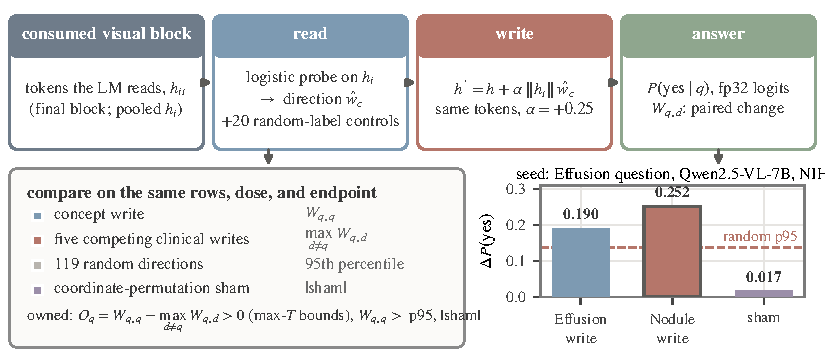
\includegraphics[width=\textwidth]{figures/fig1_framework.pdf}
    \caption{\textbf{From readable directions to semantic ownership.} A linear probe extracts named directions from the consumed visual representation and reuses them as interventions at the same block. In our patient-disjoint Qwen result, both Effusion and Nodule directions increase the Effusion answer, but Nodule is stronger. The Effusion direction remains a reproducible, non-generic writer while failing the matched clinical-family test for Effusion-specific ownership.}
    \label{fig:framework}
\end{figure*}

Our three model--concept cells on NIH ChestX-ray14 reveal two forms of reader--writer mismatch. All three cells are robustly readable, with AUROC from 0.7742 to 0.8009 and positive controlled selectivity; the paired selectivity contrasts do not resolve an ordering. The LLaVA directions do not satisfy the same generic-control criterion, whereas Qwen Effusion does so twice, including on the patient-disjoint 400-patient cohort. It is a large, reproducible, non-generic write effect whose specific Effusion attribution breaks under semantic competition because the maximum over five fixed clinical alternatives is reliably larger. We then test the implied mechanism prospectively: a full six-direction by six-question matrix finds neither a named owner nor a shared alias beyond 119 random directions, and a fresh within-patient Consolidation experiment does not close the measured input gap beyond its controls.

Our contributions are threefold. First, we formulate probe-vector interpretation as a reader--writer identification problem and introduce \emph{semantic competition}: comparing the named normal with equally constructed clinical alternatives at one consumed representation. Second, we show that robust readers need not become selective writers, and that a writer which beats random and sham controls need not be specific to its read label. Third, we follow that mismatch through two prospective mechanism gates: a complete matched clinical response surface and an input-displacement closure test. Both preserve the attribution boundary rather than recovering a concept-specific causal mechanism.

The practical principle is simple: non-semantic controls support a non-generic effect under the registered comparison, while semantic competitors and mechanism tests determine what, if anything, makes it clinically specific. Sections~\ref{sec:related}--\ref{sec:protocol} place and define these tests, Section~\ref{sec:results} follows the evidence from intervention efficacy through mechanism confirmation, and Sections~\ref{sec:discussion}--\ref{sec:conclusion} develop its implications and scope.
